\documentclass[11pt,twoside]{article}
\usepackage{setspace,amssymb,latexsym,amsmath,amscd,epsfig,amsthm}
\usepackage{array,color,booktabs}
\usepackage[english]{babel}
\usepackage[body={6.0in, 8.2in},left=1.25in,right=1.0in]{geometry}
\usepackage[pdftex,pdfauthor={Andrew P. Acosta}, pdftitle={Debt Portfolio Cash Flow at Risk},pdfsubject={CFaR},pdfdisplaydoctitle={true},pdffitwindow={true},colorlinks]{hyperref}

\newcommand{\nucl}[3]{%
  \ensuremath{%
    \phantom{\ensuremath{^{#1}_{#2}}}%
    \llap{\ensuremath{^{#1}}}%
    \llap{\ensuremath{_{\rule{0pt}{.75em}#2}}}%
    \mbox{#3}%
  }%
}

\numberwithin{equation}{section}

\begin{document}
\title{Debt Portfolio Cash Flow at Risk}
\author{Andrew P. Acosta}
%\date{}

\maketitle
\abstract{For the debt portfolio cash flow at risk prototype, I calculate the cost of refinancing existing debt at maturity date based on randomly forecast interest rates. I generate 500 normally-distributed random walk rate changes of the current coupon for each instrument in the portfolio using a driftless mean and volatility obtained from a public source. This ignores yield curve correlation because it assumes all rates are equally sensitive to changes. The analysis ultimately created a confidence interval for all years where Exelon has a bond debt exposure.} \\
{\tiny Document typeset using \AmS{}-\LaTeX{} on \today{}.}

\section{Problem}
Exelon has a number of fixed-income obligations that may be refinanced in the future at interest rates obtained at the date of the previous bond's maturity. Because the interest rate environment at that time is uncertain, a cash flow risk is introduced.

The problem is to construct a model that should produce an ``at risk" amount based on the mean and the 5th percentile for changes in interest rates, as well as the sensitivity to a LIBOR shock up or down of 300 bps.  I started by working with the Treasury team to get an updated view on our debt portfolio.  From that data, I created a simple text file that had some basic information about the bonds sufficient to make estimates about the refinancing risk.

Next, I created a prototype in the R environment. I pulled volatilities and interest rate yield curves from a Bloomberg Terminal.   The model will measure the impact of future debt maturities on existing fixed rate debt.  

If we use Towers Perrin's system for modeling pension funds, this prototype will give us something against which to compare our valuation.  It will also give us a general idea of the magnitude of our sensitivity to interest rates for purposes of prioritizing this piece of the cash flow at risk project.

\section{Data}
I have a listing of the current debt portfolio in Table~\ref{tab:debt_portfolio}. For now, I will ignore any optionality and ``make whole" agreements because it adds complexity which can be added on later. To do so requires an element of sinking fund and call schedules (which may be obtained from Bloomberg given a proper CUSIP).

\begin{table}[htbp]
	\centering
	\begin{tabular}{crrrr}
	\toprule
	\multicolumn{5}{c}{Exelon Treasury Debt Portfolio} \\
	\hline
CUSIP & Maturity & Term & Debt Outstanding & Coupon \\
\hline
\textit{none} & 2009 &	9 &	9,860,950 & 6.330 \\
705220AL5 &	2009 &	9 &	91,447,744	& 7.650 \\
30161NAB7 &	2010 &	5 &	400,000,000	& 4.450 \\
202795HJ2 &	2010 &	7 &	212,000,000	& 4.740 \\
705220AM3 &	2010 &	9 &	805,460,000	& 6.520 \\
202795HP8 &	2011 &	5 &	345,000,000	& 5.400 \\
30161MAB9 &	2011 &	10 &	699,975,000	& 6.950 \\
30161NAA9 &	2011 &	10 &	500,000,000	& 6.750 \\
693304AB3 &	2011 &	10 &	250,000,000	& 5.950 \\
202795AW0 &	2011 &	50 &	3,200,000	& 4.750 \\
246015BL4 &	2012 &	4 &	150,000,000	& 4.000 \\
202795HE3 &	2012 &	10 &	450,000,000	& 6.150 \\
693304AD9 &	2012 &	10 &	225,000,000	& 4.750 \\
693304AM9 &	2013 &	5 &	300,000,000	& 5.600 \\
202795FJ4 &	2013 &	20 &	125,000,000	& 7.625 \\
202795FM7 &	2013 &	20 &	127,000,000	& 7.500 \\
\hline
693304AN7 &	2014 &	5 &	250,000,000	& 5.000 \\
30161MAD5 &	2014 &	11 &	500,000,000	& 5.350 \\
451888CQ2 &	2014 &	20 &	17,000,000	& 5.850 \\
30161NAD3 &	2015 &	10 &	800,000,000	& 4.900 \\
202795HH6 &	2015 &	12 &	260,000,000	& 4.700 \\
202795HN3 &	2016 &	10 &	415,000,000	& 5.950 \\
202796HS2 &	2017 &	10 &	425,000,000	& 6.150 \\
30161MAE3 &	2017 &	10 &	700,000,000	& 6.200 \\
202795HU7 &	2018 &	10 &	700,000,000	& 5.800 \\
693304AL1 &	2018 &	10 &	500,000,000	& 5.350 \\
202795GX2 &	2018 &	20 &	140,000,000	& 6.950 \\
61360QAA  &	2028 &	30 &	78,105,000	& 7.380 \\
20035AAA2 &	2033 &	30 &	200,000,000	& 6.350 \\
202795HG8 &	2033 &	30 &	253,600,000	& 5.875 \\
693356AA3 &	2033 &	30 &	100,000,000	& 5.750 \\
693304AG2 &	2034 &	30 &	75,000,000	& 5.900 \\
30161NAC5 &	2035 &	30 &	500,000,000	& 5.625 \\
202795HK9 &	2036 &	30 &	625,000,000	& 5.900 \\
693304AH0 &	2036 &	30 &	300,000,000	& 5.950 \\
693304AJ6 &	2037 &	30 &	175,000,000	& 5.700 \\
202795HT0 &	2038 &	30 &	450,000,000	& 6.450 \\
	\bottomrule
	\end{tabular}
	\caption{Bond portfolio of fixed-rate coupon paying instruments sorted by maturity year and coupon. Only the bonds with maturities between 2009--2013 are modeled for refinancing analysis so that results are compliant with five-year LRP.}
	\label{tab:debt_portfolio}
\end{table}



\section{Assumptions}
In order to proceed in creating a prototype, and to add on functionality piece-by-piece, I make a few assumptions about the data and the analysis leading to a CFaR estimate.
\begin{enumerate}
\item I will ignore any optionality and ``make whole" agreements at first. This adds an element of sinking fund and call schedules.
\item I will ignore differences in day-count convention, and assume all bonds are actual/actual, although some are 30/360.
\item The credit spread above benchmark rate is unknown, and will be assumed to be a random variable with a mean set to be the muni rate spread for a BBB general obligation bond (Bloomberg yield curve: M631) of similar tenor. Corporate bonds will also be assumed to be a random variable with a mean set to be the BBB corp curve rate (Bloomberg yield curve: C041).
\item When refinancing debt, I will be calculating the cost based on its principal as of my data set April 31, 2009. \emph{Debt is refinanced only once}.
\item Floating rate debt and fixed-to-floating swaps are not part of this prototype because either their interest rate risk is minimal, or would introduce complexity that should be deferred to later developments.
\item I use a constant spread for corporate bonds that does not differ by tenor. This is easily modified by obtaining bond spread statistics from Bloomberg and entering them into the pricing algorithm.
\item I am modeling a single interest rate point, and not the dynamics of the yield curve, which uses methods explained in Section~\ref{multifactor}.
\end{enumerate}

\section{Analysis}
Our interest rate generator is a simple one. We use a Vasicek model, % (Brigo, p. 50)
\begin{equation}
dr(t)=\underbrace{k[\theta-r(t)]dt}_{\text{mean reversion}} + \overbrace{\sigma dW(t)}^{\text{volatility}}, \quad r(0)=r_0.
\label{eq:vasicek}
\end{equation}
where $r_0$, $k$, $\theta$, and $\sigma$ are positive constants. When we integrate \eqref{eq:vasicek}, we have our rate generator,
\begin{equation}
r(t)=r(s)e^{-k(t-s)} + \theta \big( 1-e^{-k(t-s)} \big) + \sigma \int^t_s e^{-k(t-u)} dW(u).
\label{eq:vasicek_integrated}
\end{equation}

Further developments may require a more sophisticated model since Vasicek does not have reliable mean reversion and does not always produce positive interest rates. With a more sophisticated model, we may also simulate option pricing of any embedded optionality in the bonds,
\begin{equation}
V(t)=P(t,S) \phi(d_1)- K P(t,T) \phi(d_2)
\label{eq:vasicek_option}
\end{equation}
where
\begin{eqnarray*}
d_1 &=& \frac{1}{\sigma_p} \log \frac{P(t,S)}{KP(t,T)} + \frac{\sigma_p}{2}, \quad d_2=d_1-\sigma_p, \\
\sigma_p &=& \frac{\sigma}{\alpha} \big(1-\text{e}^{-\alpha(S-T)} \big) \sqrt{\frac{1-\text{e}^{-2 \alpha(T-t)}}{2\alpha}}.
\end{eqnarray*}

We begin with 500 trials of a random interest rate path. An example of these rate paths is depicted in Figure~\ref{figure:rate_path_set}. The starting point of \eqref{eq:vasicek_integrated} and the amount of variance is obtained from observations of the actual market at the time of CFaR analysis. A similar procedure would be required for \eqref{eq:vasicek_option}.
\begin{figure}[tbh]
  \centering
  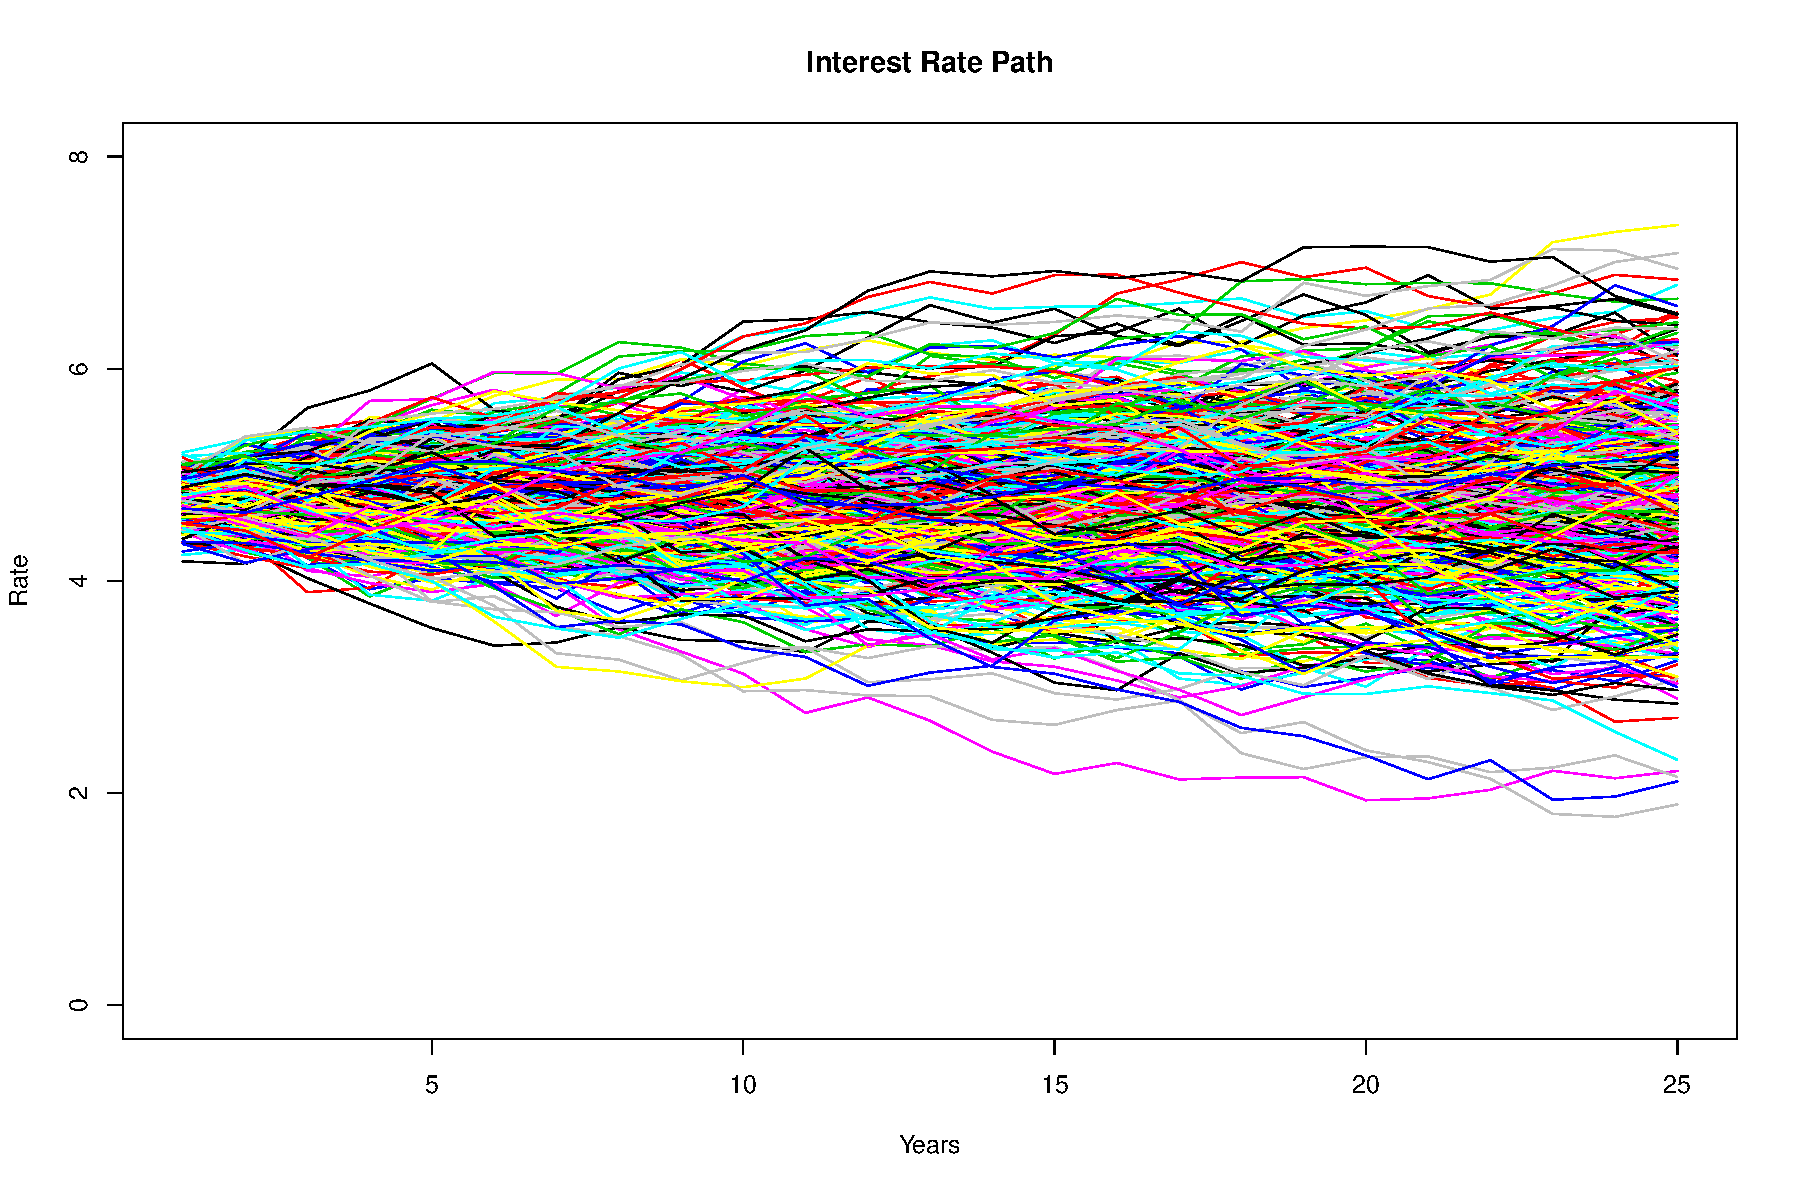
\includegraphics[scale=.5]{rate_path_set}
  \caption{A possible set of the evolution of spot rate paths based upon observed conditions in the BBB corporate bond market.}
  \label{figure:rate_path_set}
\end{figure}

\subsection{Simulation}\label{simulation}
The 500 trials, which represent 500 different rate simulations, step through time for 25 years, which is the length of time of our longest maturity bond (5 years) plus its term (20 years). Each bond is priced at its maturity date using a simulated interest rate appropriate to its time forward plus a BBB corporate bond spread, which for this prototype was held at 250 bps. For instance, a bond maturing in 2013 would be priced at a simulated rate that is 5 years out.

The difference between the previous coupon and the sum of the simulated rate and spread is multiplied by the debt outstanding. 
\begin{equation}
(\textit{Previous Coupon}  - \textit{Simulated Rate} + \textit{BBB Corp. Spread}) \times \textit{Debt Outstanding}
\label{eq:cfar_delta}
\end{equation}
This difference is the cash flow at risk for this bond. The routine \eqref{eq:cfar_delta} is repeated 500 times, and its results summed in the appropriate years. The number of cash flow differences is determined by the bond's term. So, for example, a ten-year bond would have 500 simulations of ten consecutive cash flow differences starting at the current bond's maturity year.

When all simulations are run for all bonds, we have 500 sets of cash flow differences going out for 25 years, however, we are only concerned with a five-year LRP. Pricing the debt portfolio gives us Figure~\ref{figure:box_plots}.
\begin{figure}[thb]
  \centering
  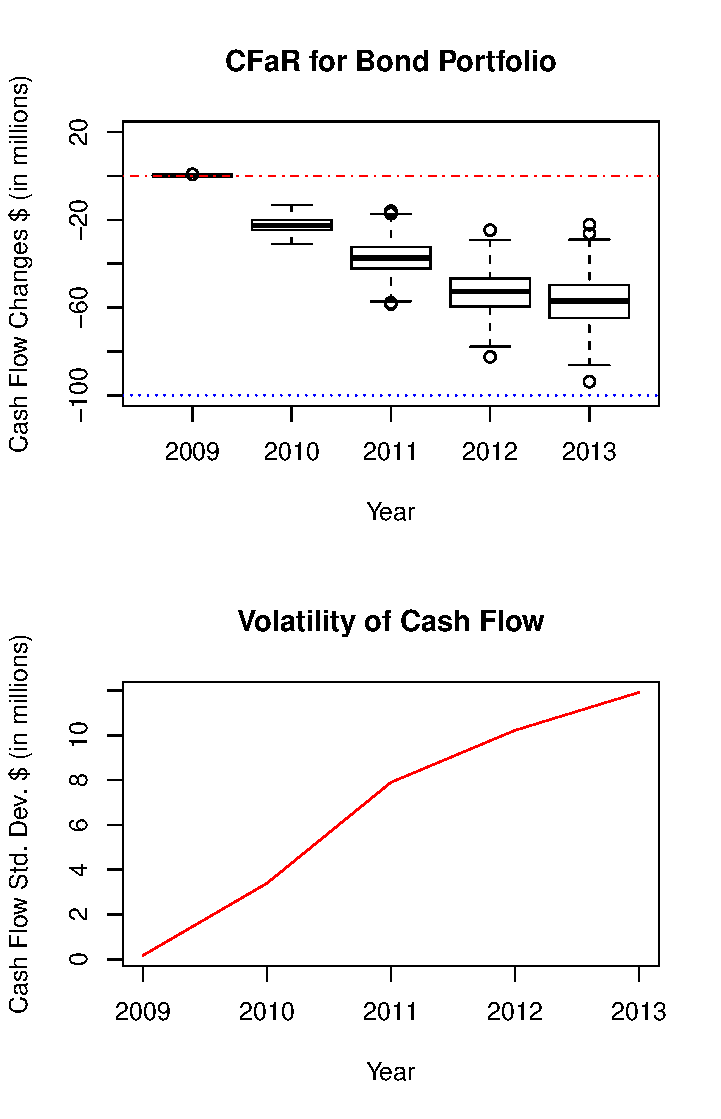
\includegraphics[scale=.65]{box_plots}
  \caption{Box and whisker plots of CFaR for each of debt exposure. Below it, is the volatility of cash flows, which follows a very similar pattern from the box and whisker plots.}
  \label{figure:box_plots}
\end{figure}

\subsection{Finding CFaR}
The top panel of Figure~\ref{figure:box_plots} gives us the cash flow at risk for each individual year. If we look at the entire LRP horizon collectively, as seen in Figure~\ref{figure:cfar_density}, we get an estimate of the cash flow uncertainty.
\begin{figure}[t]
  \centering
  \includegraphics[scale=.45]{cfar_density}
  \caption{Probability density estimate of CFaR for five-year LRP period. Also depicted is the actual histogram of cash flow changes.}
  \label{figure:cfar_density}
\end{figure}

\section{Deterministic Rate Shocks}
Instead of measuring interest rate changes using a stochastic rate evolution model like the one in Section~\ref{simulation}, we could use a deterministic interest rate shock that instantaneously will increase or decrease the coupon rate. The interest rate sensitivities by year are listed in Table~\ref{tab:rate_shocks}. The grand total of 100 bps sensitivities for all five years is \$419,196,683.

\begin{table}[h]
	\centering
	\begin{tabular}{cr}
	\toprule
	\multicolumn{2}{c}{Exelon Treasury Debt Portfolio Sensitivities} \\
	\hline
Maturity & \$ Shock \\
\hline
2009 & \$9,117,783 \\
2010 & \$107,331,400 \\
2011 & \$163,847,500 \\
2012 & \$73,500,000 \\
2013 & \$65,400,000	\\
%\hline
%Total & \$419,196,683 \\
\bottomrule
	\end{tabular}
	\caption{Bond portfolio rate sensitivity to a 100 bps rate shock to fixed-rate coupon paying instruments.}
	\label{tab:rate_shocks}
\end{table}



\section{Future Enhancements}
\subsection{Mean-Reversion Models}
For interest rates, a mean-reversion model has more economic logic than the Vasicek model presented in \eqref{eq:vasicek}.
Suppose that an interest rate follows a geometric mean-reverting process,
\begin{equation}
dP = h P (M -  P) dt + s P dz
\label{eq:mean_reversion}
\end{equation}
Where $P$ is the long-run equilibrium level (\emph{or the long-run mean interest rate which the prices tend to revert}); and $h$ is the speed of reversion. The others terms have the same meaning of \eqref{eq:vasicek_integrated}, presented before. There are numerous enhancements to \eqref{eq:mean_reversion} to fit specific interest rate assumptions.

\subsection{Multifactor Interest Rate Models}\label{multifactor}
I will obtain the interest rate volatility of each relevant term point (maybe 8 to 10 term points) and a correlation matrix between term points. From that, I can get the eigenvectors to create a transformed matrix of yield curve factors and sensitivities. While being more complex, this acknowledges that the entire yield curve may behave differently at certain tenors.

To demonstrate using principal component analysis\index{principal component analysis} and eigenvalue decomposition\index{eigenvalue decomposition} in Monte Carlo simulation of a yield curve comprising several fixed income instruments, we turn to an example % in \cite{marrison2002frm}.
To begin, consider a U.S. government yield curve. We have statistics in the following matrices: standard deviation $\mathbf{S}$, correlation $\mathbf{R}$, and covariance $\mathbf{C}$ for absolute changes in the 3-month, 1-year, 5-year, and 20-year interest rates. Using these matrices, we want to create a matrix $\mathbf{B}$ that will assist us in creating random scenarios.

\begin{eqnarray*}
\mathbf{S} &=&
\begin{bmatrix}
	0.051 & 0.052 & 0.061 & 0.054
\end{bmatrix} \\
\\
\mathbf{R} &=&
\begin{bmatrix}
	1 & 0.61 & 0.42 & 0.31 \\
	0.61 & 1 & 0.83 & 0.67 \\
	0.42 & 0.83 & 1 & 0.88 \\
	0.31 & 0.67 & 0.88 & 1
\end{bmatrix} \\
\\
\mathbf{C} &=& diag(\mathbf{S}) \times \mathbf{R} \times diag(\mathbf{S}) \\
\\
&=&
\begin{bmatrix}
	.0026 & .0016 & .0013 & .0008 \\
	.0016 & .0027 & .0026 & .0019 \\
	.0013 & .0026 & .0038 & .0029 \\
	.0008 & .0019 & .0029 & .0029
\end{bmatrix}.
\end{eqnarray*}
We obtain the eigenvalue decomposition of $\mathbf{C}$ in MATLAB or Octave using,
\begin{verbatim}
    lambda_sqrt = sqrt(eig(C));
    eigv_decom=diag(lambda_sqrt)
\end{verbatim}

\begin{equation}
\mathbf{\Lambda}^{1/2}=
\begin{bmatrix}
	0.017804 & 0 & 0 &  0 \\
	0 & 0.024739 & 0 &  0 \\
	0 & 0 & 0.046721 & 0 \\
	0 & 0 & 0 & 0.094277 \\
	\label{eq:eigenfacors}
\end{bmatrix}
\end{equation}
Eigenvectors have special properties that are useful for speeding up Monte Carlo simulations. Each eigenvector, such as the diagonal that created \eqref{eq:eigenfacors}, defines a market movement that is by definition independent of the other movements, because $\mathbf{I}=\mathbf{E}^T\mathbf{E}$. Our $\mathbf{E}$ matrix is,
\begin{equation}
\mathbf{E}=
\begin{bmatrix}
	\phantom{-}0.097 & -0.480 & \phantom{-}0.724 & -0.486 \\
	\phantom{-}0.407 & -0.694 & -0.124 & \phantom{-}0.581 \\
	-0.847 & -0.195 & \phantom{-}0.264 & \phantom{-}0.417 \\
	\phantom{-}0.327 & \phantom{-}0.500 & \phantom{-}0.625 & \phantom{-}0.502 \\
	\label{eq:Ematrix}
\end{bmatrix}
\end{equation}
How do we know \eqref{eq:Ematrix} is an $\mathbf{E}$ matrix? Because \texttt{abs(round(transpose(E)*E))} makes a $4 \times 4$ identity matrix. Finally, we compute $\mathbf{B}=\mathbf{\Lambda}^{1/2} \mathbf{E}$,
\begin{equation}
\mathbf{B}=
\begin{bmatrix}
	\phantom{-}0.0017269 & -0.0085457 & \phantom{-}0.0128898 & -0.0086525 \\
	\phantom{-}0.0100687 & -0.0171688 & -0.0030676 & \phantom{-}0.0143733 \\
	-0.0395723 & -0.0091105 & \phantom{-}0.0123342 & \phantom{-}0.0194825 \\
	\phantom{-}0.0308287 & \phantom{-}0.0471387 & \phantom{-}0.0589233 & \phantom{-}0.0473272
	\label{eq:Bmatrix}
\end{bmatrix}
\end{equation}
We have four principal components, named \emph{wiggle}, \emph{flex}, \emph{twist}, and \emph{shift}. We can use the matrix $\mathbf{B}$ to create random scenarios,
\[
\begin{bmatrix}
\delta r_{3mo} & \delta r_{1yr} & \delta r_{5yr} & \delta r_{20yr}
\end{bmatrix}
=
\begin{bmatrix}
z_1 & z_2 & z_3 & z_4
\end{bmatrix}
\times \mathbf{B}.
\]
where $z_n$ is a random number generated for factor $n$. Each row of $\mathbf{B}$ describes its sensitivity to changes in the factor and the rate point,
\begin{eqnarray*}
wiggle &=& z_1 
\begin{bmatrix}
\phantom{-}0.0017269 & -0.0085457 & \phantom{-}0.0128898 & -0.0086525
\end{bmatrix}\\
flex &=& z_2
\begin{bmatrix}
\phantom{-}0.0100687 & -0.0171688 & -0.0030676 & \phantom{-}0.0143733
\end{bmatrix} \\
twist &=& z_3
\begin{bmatrix}
-0.0395723 & -0.0091105 & \phantom{-}0.0123342 & \phantom{-}0.0194825
\end{bmatrix} \\
shift &=& z_4
\begin{bmatrix}
\underbrace{\phantom{-}0.0308287}_{3mo} & \underbrace{\phantom{-}0.0471387}_{1yr} & \underbrace{\phantom{-}0.0589233}_{5yr} & \underbrace{\phantom{-}0.0473272}_{20yr}
\end{bmatrix}.
\end{eqnarray*}
We can see that for any given change in $z_n$, the \emph{shift} has the strongest effect, and \emph{wiggle} is the weakest.

For instance, if $z_4$ increases by 1, all of the rate points shift up by the magnitude of the bottom row of \eqref{eq:Ematrix}, which means the 3-month rate increases by 3 bps, the 1-year by 5 bps, the 5-year by 6 bps, and the 20-year by 5 bps. Notice that a positive change of 1 to $z_3$ would cause \emph{twist} in the 3-month rate to decrease 4 bps, and the 1-year to decrease 1 bp, but the 5- and 20-year rates increase 1 and 2 bps, respectively.

Since \emph{wiggle} and \emph{flex} have the least amount of influence, if we wanted to optimize our Monte Carlo simulation by reducing the number of random variables, we could hold $z_1$ and $z_2$ constant, and let $z_3$ and $z_4$ be random.

Imagine a process where we capture thousands of iterations of the following simulations. We will hold \emph{wiggle} and \emph{flex} constant, and will apply random shocks to \emph{twist} and \emph{shift}. We set $m$ to the magnitude of the random shock, and use \texttt{normrnd} to generate a normally-distributed random number with $\mu=0$ and $\sigma=1$.
\begin{verbatim}
    m=2
    round([1 1 m*normrnd(0,1) m*normrnd(0,1)]*(100*B))
\end{verbatim}
This gives us a row vector of basis point shocks for each rate point. For example, in one trial, the rate shocks $\delta r$ were obtained.
\[
\underbrace{-3 \text{ bps}}_{3mo} \quad \underbrace{-2 \text{ bps}}_{1yr} \quad \underbrace{6 \text{ bps}}_{5yr} \quad \underbrace{8 \text{ bps}}_{20yr}.
\]


%\bibliographystyle{apacite}
%\bibliography{msf566-notes}
\end{document} 